\documentclass[../Main.tex]{subfiles}
\begin{document}

\section{Existing Alternative Games}
In this chapter, seven different alternative games will be presented. The games are picked based on popularity, relevance today, and/or how they compare to each other. Different types of games are on purpose chosen to illustrate the diversity of alternative games that exist. In every game section, a brief explanation of the game concept and why it is an alternative game will be given.

\subsection{Hold}
Hold is an application that rewards users for not using their phones \citep{hold_hold_2020}. The game was initially launched in 2016, for iOS and Android, and the primary focus was on Norwegian university students \citep{ringheim_smarttelefon_2018}. Since then the application’s target group has expanded beyond Norwegian students. 

\begin{figure}[H]
    \begin{minipage}{.5\textwidth}
      \centering
      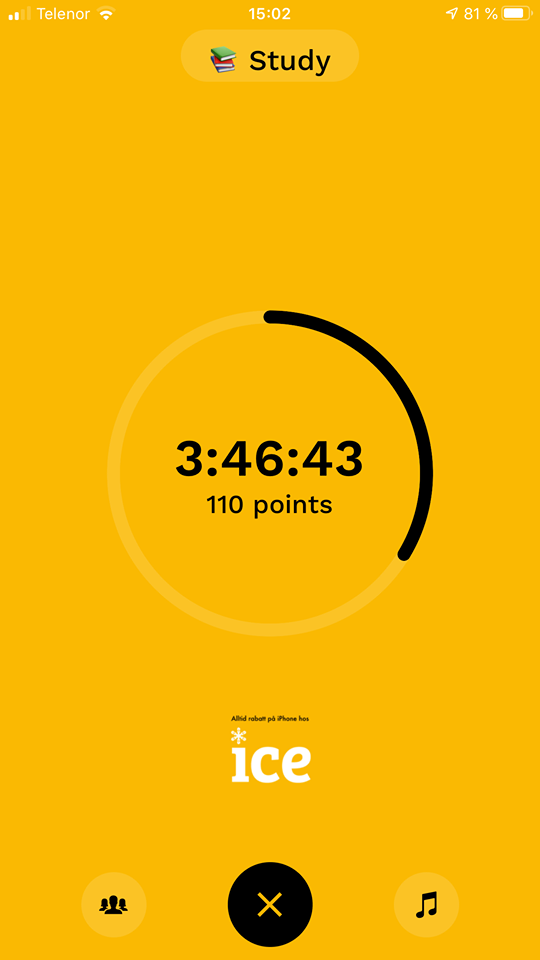
\includegraphics[width=.75\textwidth]{Images/ExistingGames/HoldApp.png}
      \captionof{figure}{Main timer screen in Hold.}
      \label{fig:hold_timer}
    \end{minipage}
    \begin{minipage}{.5\textwidth}
      \centering
      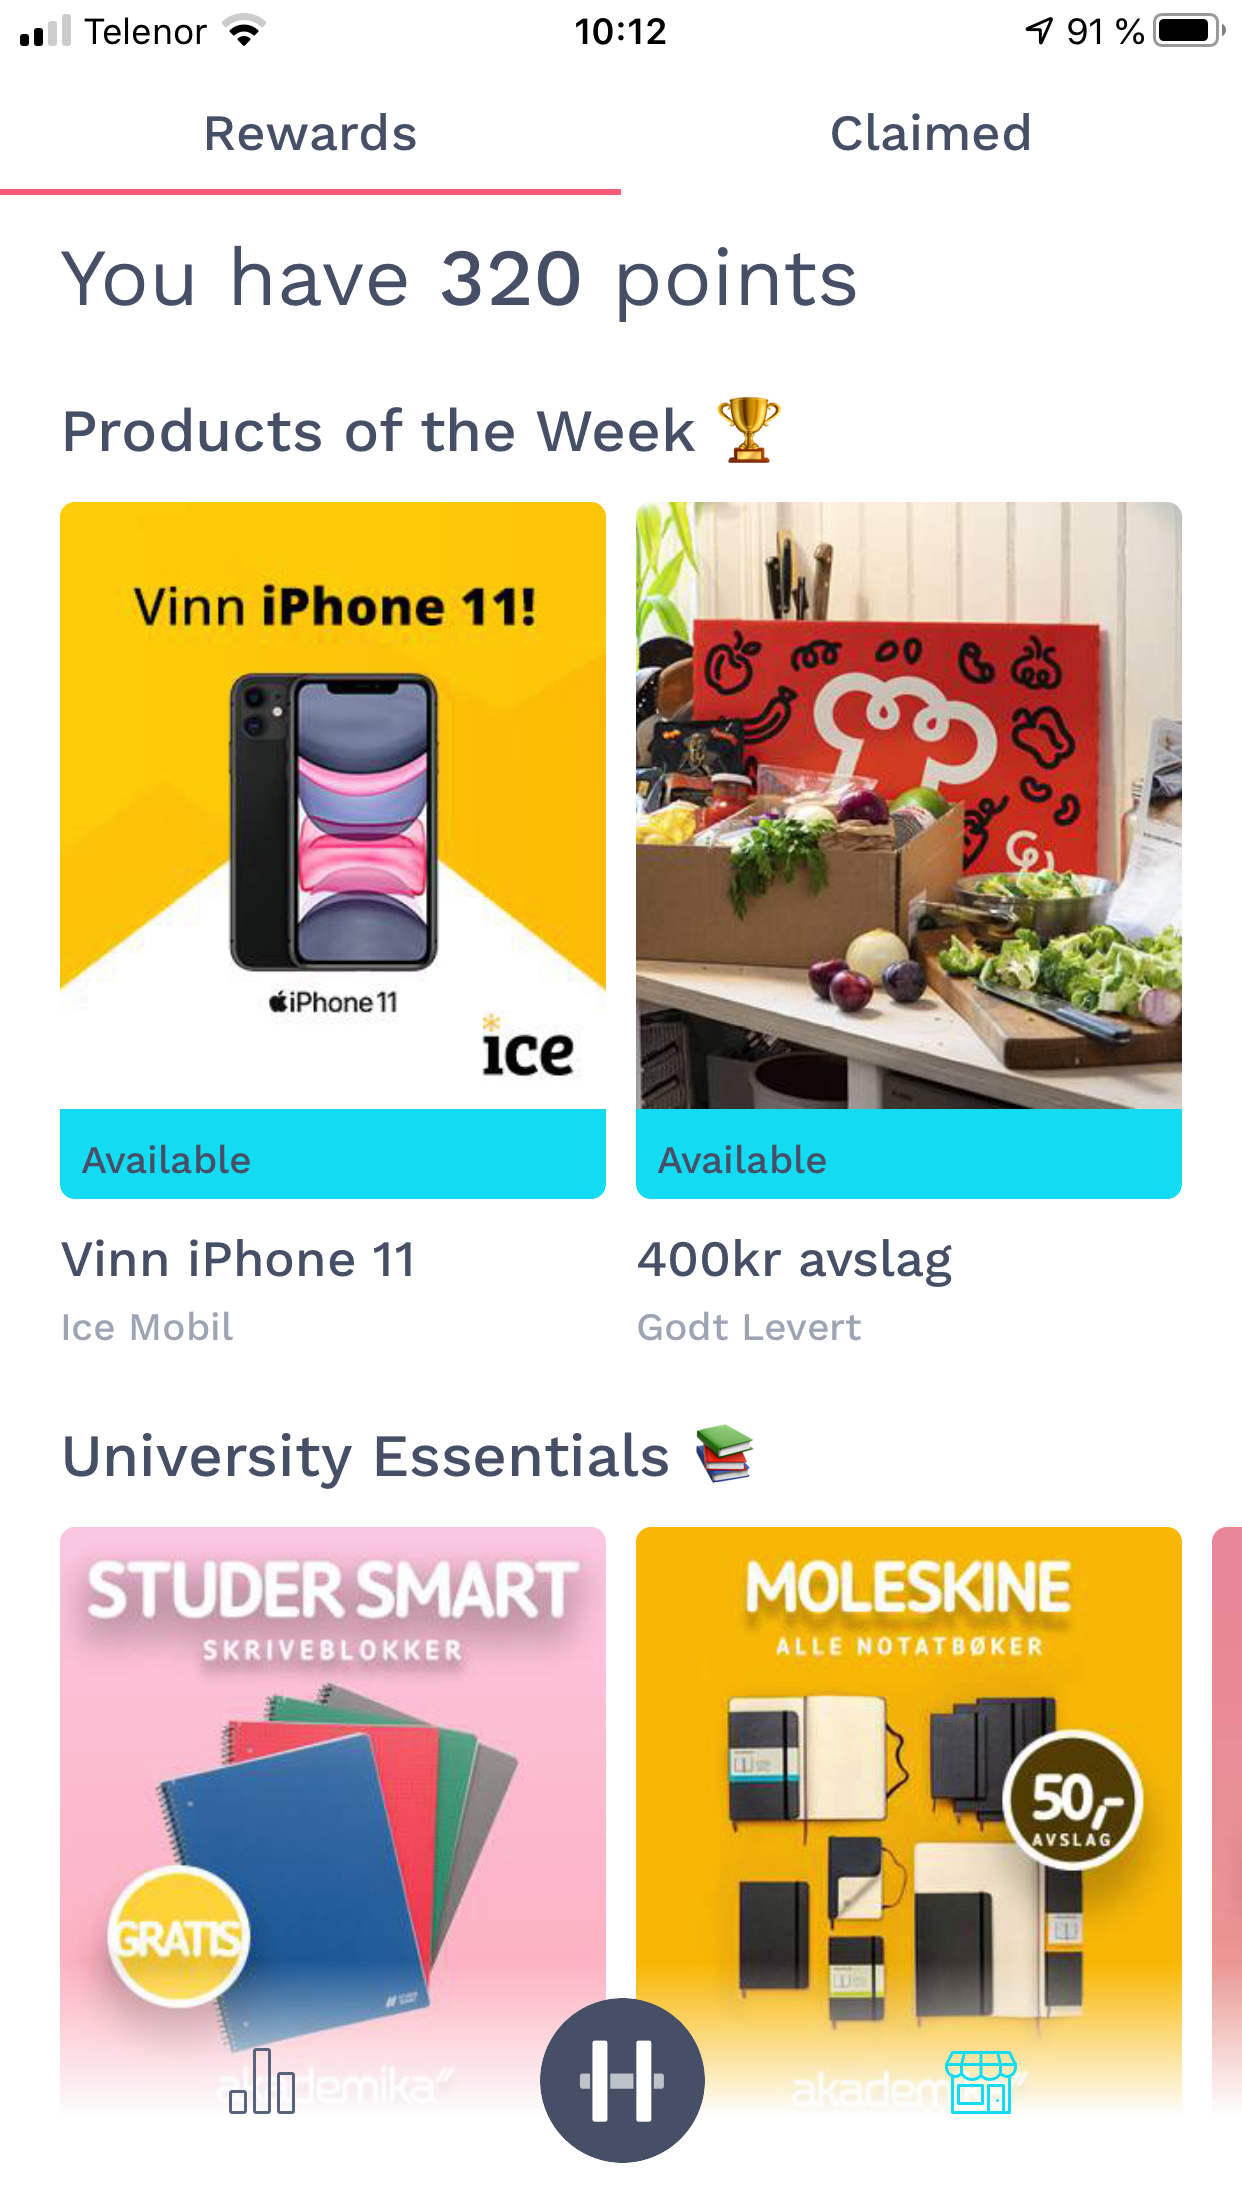
\includegraphics[width=.75\textwidth]{Images/ExistingGames/HoldAppRewards.png}
      \captionof{figure}{Choices of rewards in Hold.}
      \label{fig:hold_reward}
    \end{minipage}
\end{figure}

The application helps users limit distractions through gamification. When users activate the application, a timer starts running (see figure \ref{fig:hold_timer}). The user is rewarded with ten points for each twentieth minute they are not using their phone. The points can later be exchanged into real-life items such as coffee, food, or discounts as seen in figure \ref{fig:hold_reward}. The rewards are the main motivating factor for using the application.

Unlike other games, Hold’s concept is to encourage people to not use their mobile phones. The user can choose to play alone against the environment (PvE), or connect with friends to compare scores, which makes it more of a competitive game (PvP). The application does also let users connect with nearby friends, through Bluetooth, which enables them to collectively focus (collaborate) while boosting their points \citep{wakefield_free_2018}.

Hold is a perfect example of an alternative game with a different concept, where the developers have explored multiple of the game characteristics categories. The game classifies as an alternative primarily for two reasons: It explores alternative game genres by using gamification, rewarding the user points for not using their phone. And it uses alternative input sources, primarily Bluetooth, for connecting with nearby friends.

\subsection{Mario Kart Live}
Mario Kart Live is a newly developed augmented reality concept from Nintendo (released 16th October 2020). The game is based around the classic Mario Kart game, but with a rather unique twist: the inclusion of a specially designed RC kart that follows the user’s maneuvers in-game. A live video feed from the racing kart is relayed to the user’s Switch, mapping the virtual track to the user’s home \citep{velazco_race_2020}. The game can be played both individually (against AIs) or as a multiplayer game with more than one kart \citep{hashimoto_mario_2020}.

The game is a typical example of how an alternative game can bring something new to an already familiar game concept by using alternative input and output sources. Below (\ref{fig:mario_kart_live}) is a poster from the game where you can see the karts racing a user’s home and how the game is presented to the player. 

\begin{figure}[H]
    \centering
    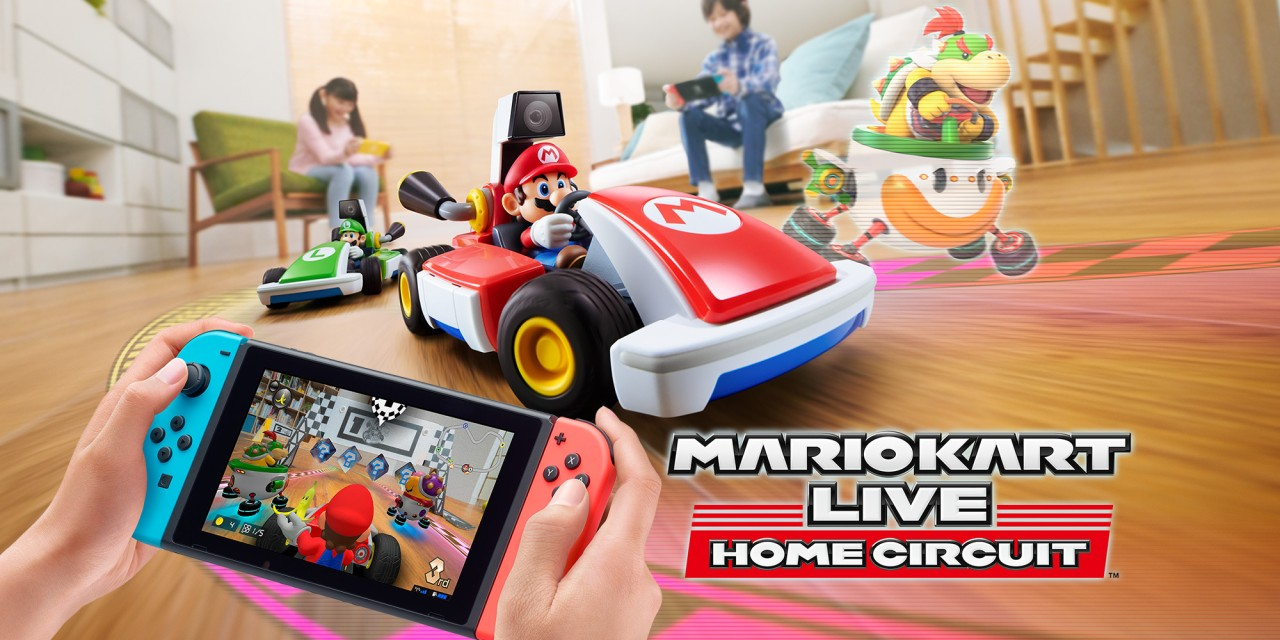
\includegraphics[width=0.8\textwidth]{Images/ExistingGames/MarioKartLive.jpeg}
    \caption{Mario Kart Live poster showing illustrated gameplay.}
    \label{fig:mario_kart_live}
\end{figure}

\subsection{Pokemon Go}
Pokémon Go is another good alternative game example, published and developed by Niantic for iOS and Android. The game was launched in 2016 and quickly became one of the most popular mobile games of all time \citep{grubb_pokemon_2016}. The concept is an extension of the classic Pokémon game found on multiple of Nintendo's handheld devices. 

\begin{figure}[H]
    \begin{minipage}{.48\textwidth}
      \centering
      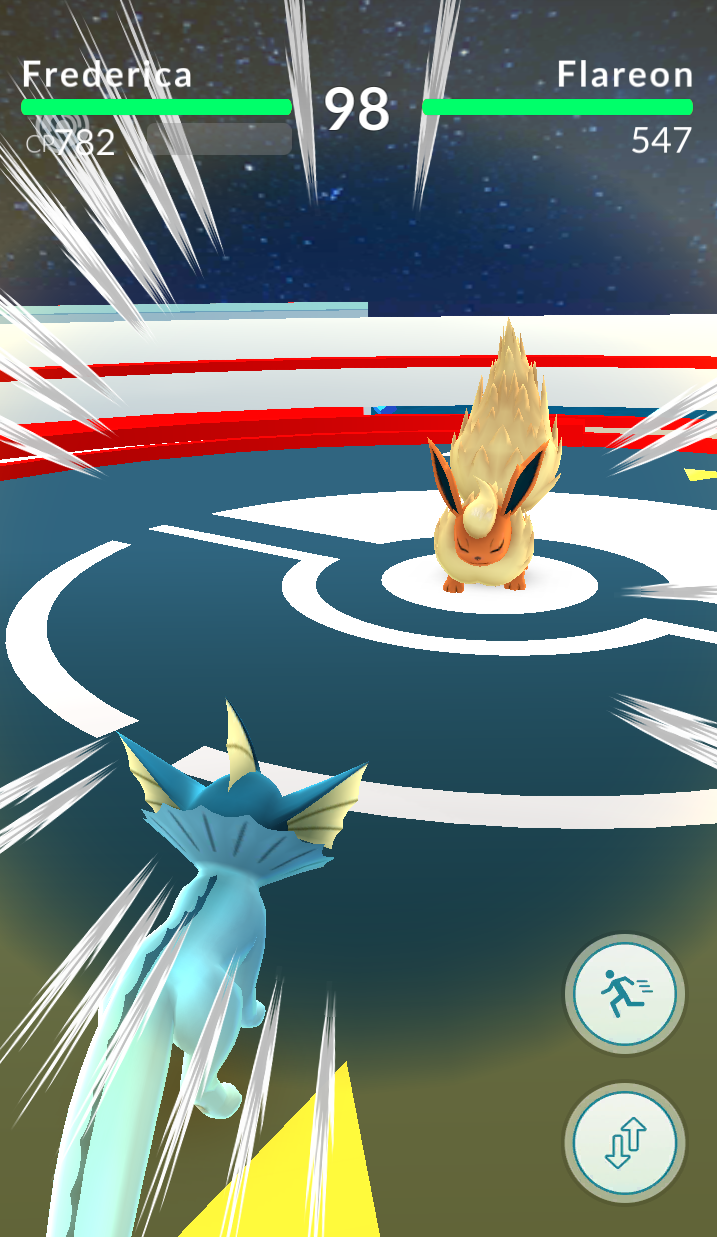
\includegraphics[width=.8\textwidth]{Images/ExistingGames/PokemonGoBattle.png}
      \captionof{figure}{Screenshot of an ongoing battle in Pokemon Go}
      \label{fig:pokemon_go_battle}
    \end{minipage}
    \hspace{0.5cm}
    \begin{minipage}{.48\textwidth}
      \centering
      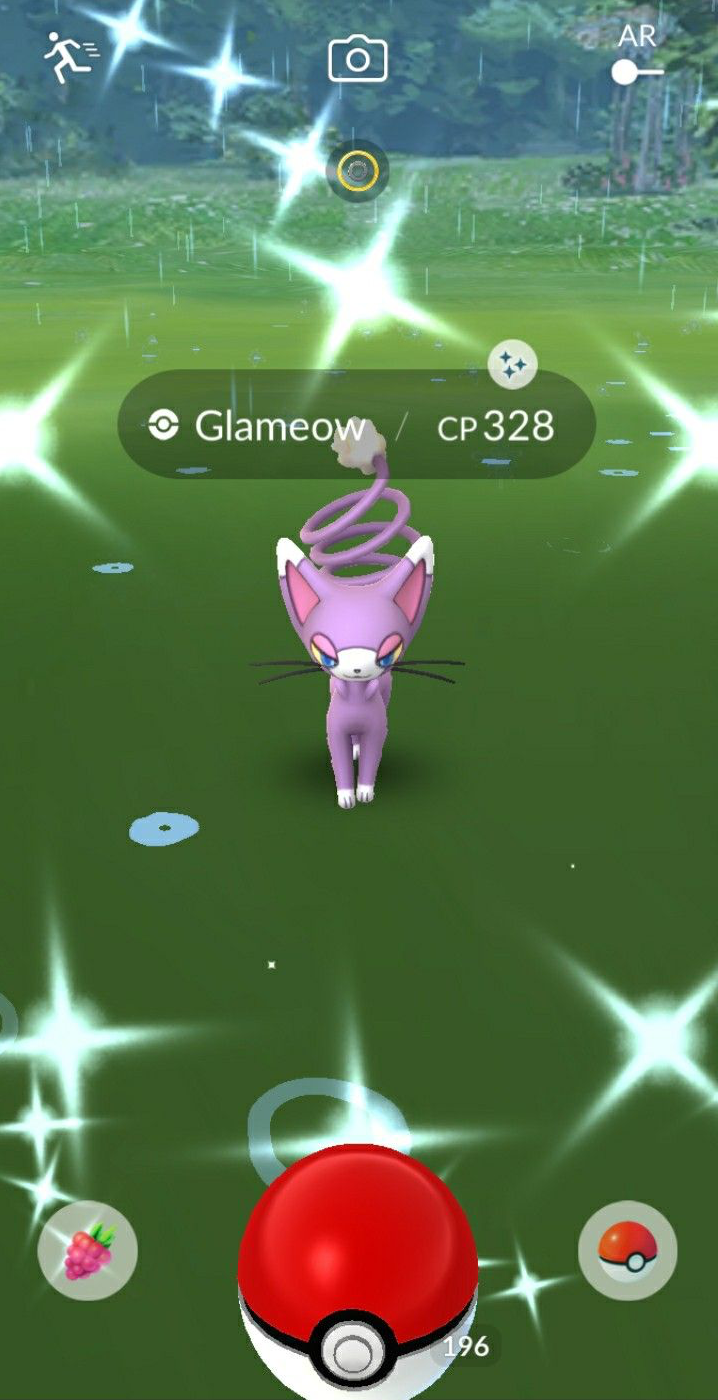
\includegraphics[width=.7\textwidth]{Images/ExistingGames/PokemonGoCatch.png}
      \captionof{figure}{Typical screenshot of gameplay in Pokemon Go.}
      \label{fig:pokemon_go_catch}
    \end{minipage}
\end{figure}

The concept is similar to the previous Pokémon games but utilizes AR and location determination (GPS) for the player to find and catch Pokémons. The player needs to move around in the real world to play the game. Battles between Pokémons (to increase combat points and get prices) can happen at specific places known as Pokémon Gyms. These spots correspond to real-world points of interest (POI) such as parks and tourist attractions \citep{bastow_pokestops_2016}. There are also additional important POI in the game, e.g. PokéStops and Nests. Figure \ref{fig:pokemon_go_battle} is an in-game screenshot where you can see a typical Pokémon battle, while figure \ref{fig:pokemon_go_catch} shows a screenshot of gameplay while catching a Pokémon.

The game is clearly an alternative game as it explores uncommon input and output sources such as camera, GPS, and AR. Pokémon Go is a good example of how alternative games can become very successful. 

\subsection{Just Dance Now}
\begin{figure}[H]
    \centering
    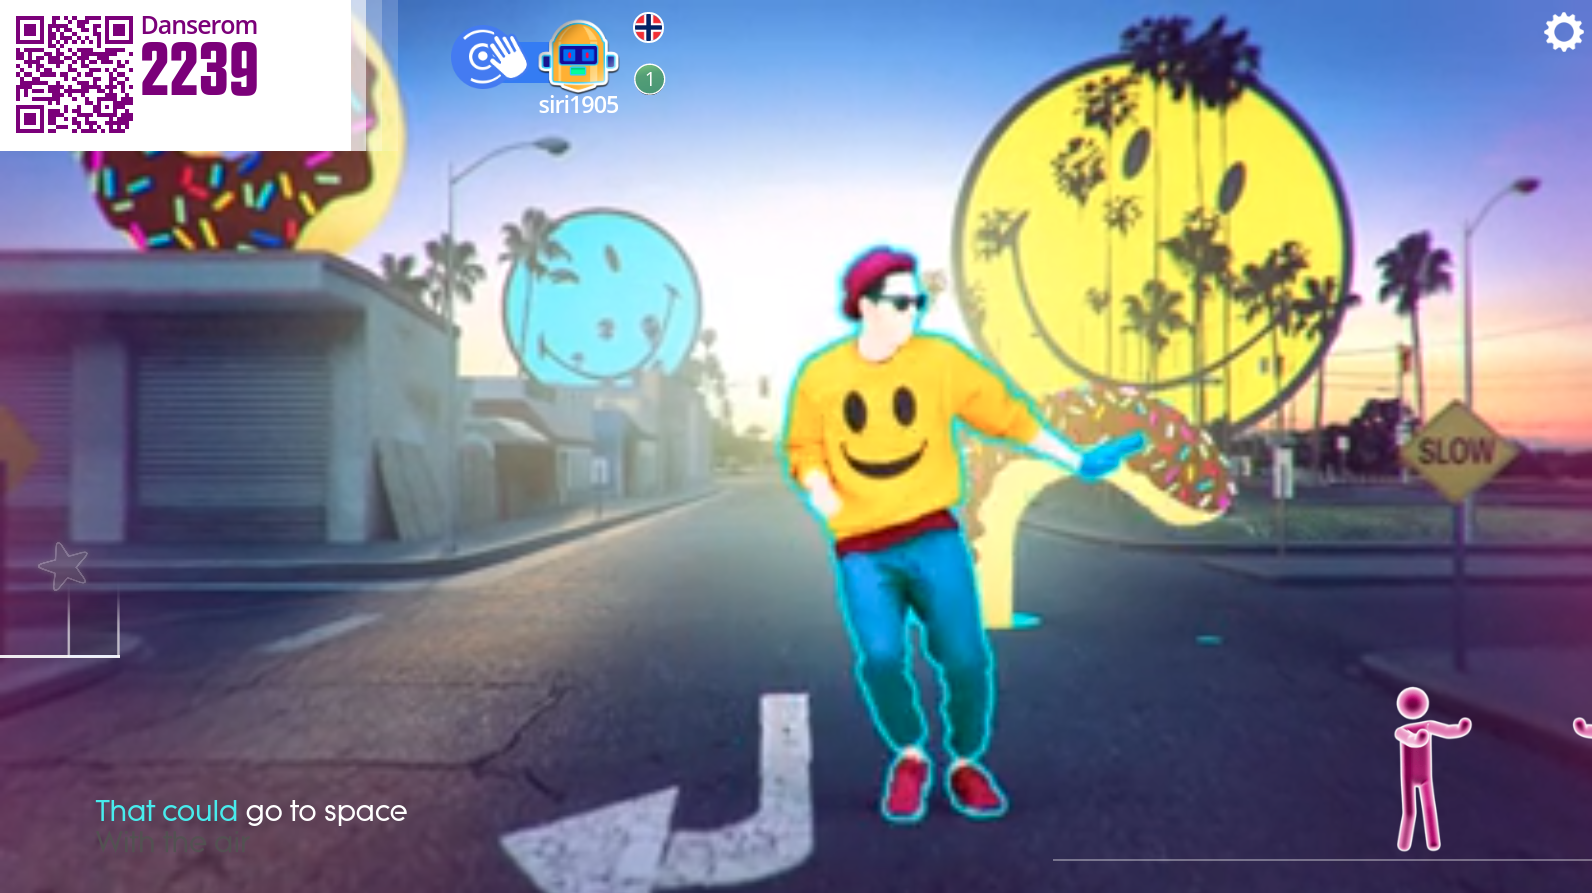
\includegraphics[width=.8\textwidth]{Images/ExistingGames/JustDanceNow_Pc.png}
    \caption{Just Dance Now screenshot from a computer screen}
    \label{fig:just_dance_now_pc}
\end{figure}

\begin{wrapfigure}{r}{0.45\textwidth}
  \begin{center}
    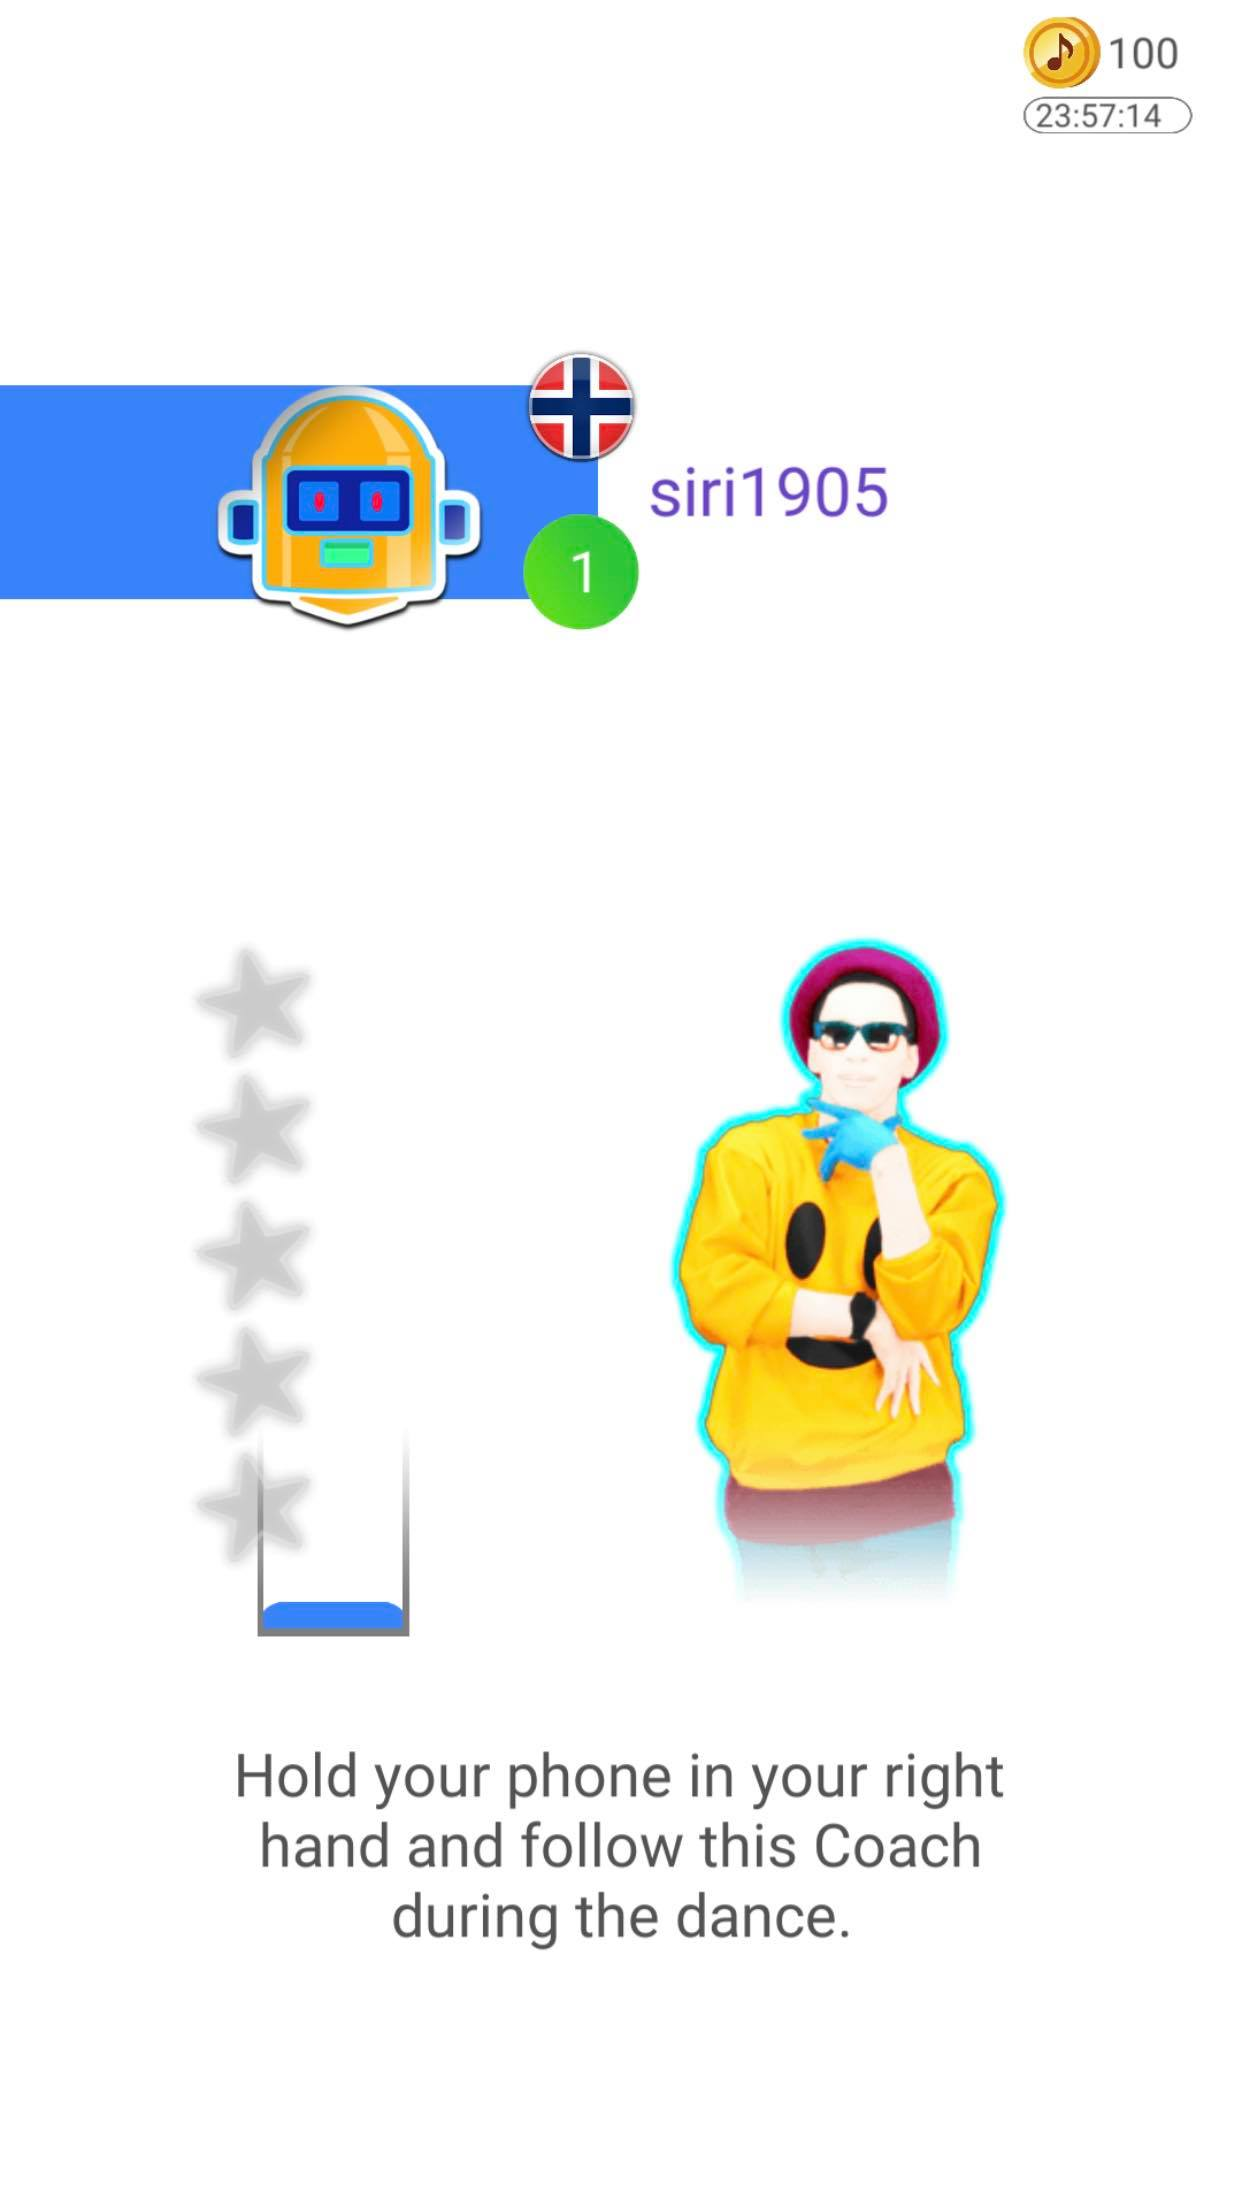
\includegraphics[width=0.40\textwidth]{Images/ExistingGames/JustDanceNow_Mobile.jpg}
  \end{center}
  \caption{figure}{Just Dance Now screenshot from Mobile}
  \label{fig:just_dance_now_mobile}
\end{wrapfigure}

Just Dance Now is an alternative game produced by Ubisoft that launched in 2014 \citep{fandom_just_2020}. The game is an addition to the Just Dance franchise, where the concept is to pick a song from the catalog and follow the moves of the on-screen character as seen in figure \ref{fig:just_dance_now_pc}.

Just Dance Now distinguishes itself from the other games in the franchises by being more available because it does not require a dedicated gaming console. It can be played using your smartphone (iOS or Android) as the controller and a large screen connected to the internet (computer, AppleTV, Chromecast, etc.) \citep{ubisoft_support_general_2020}. Your smartphone is used as a movement tracker and the large screen displays the dance moves you should perform. Multiple players can join the same game and dance together, competing, trying to get the highest score.

The main reason this game can be seen as an alternative game is the use of the player’s mobile phone as a movement tracking device, as seen in figure \ref{fig:just_dance_now_mobile}. Based on the measurements from the sensors in the player’s phone, the game determines whether or not the player is doing the dance moves well.

The interaction form is another reason why this game is an alternative game. The game is a concrete example of a Multiplayer On One Screen Entertainment System (MOOSES), presented in chapter \ref{chap:5}. All players in one game use the same large screen to see the moves they need to perform in order to get points in the game.
        
\subsection{Guitar Hero}
\begin{wrapfigure}{r}{0.45\textwidth}
    \begin{center}
        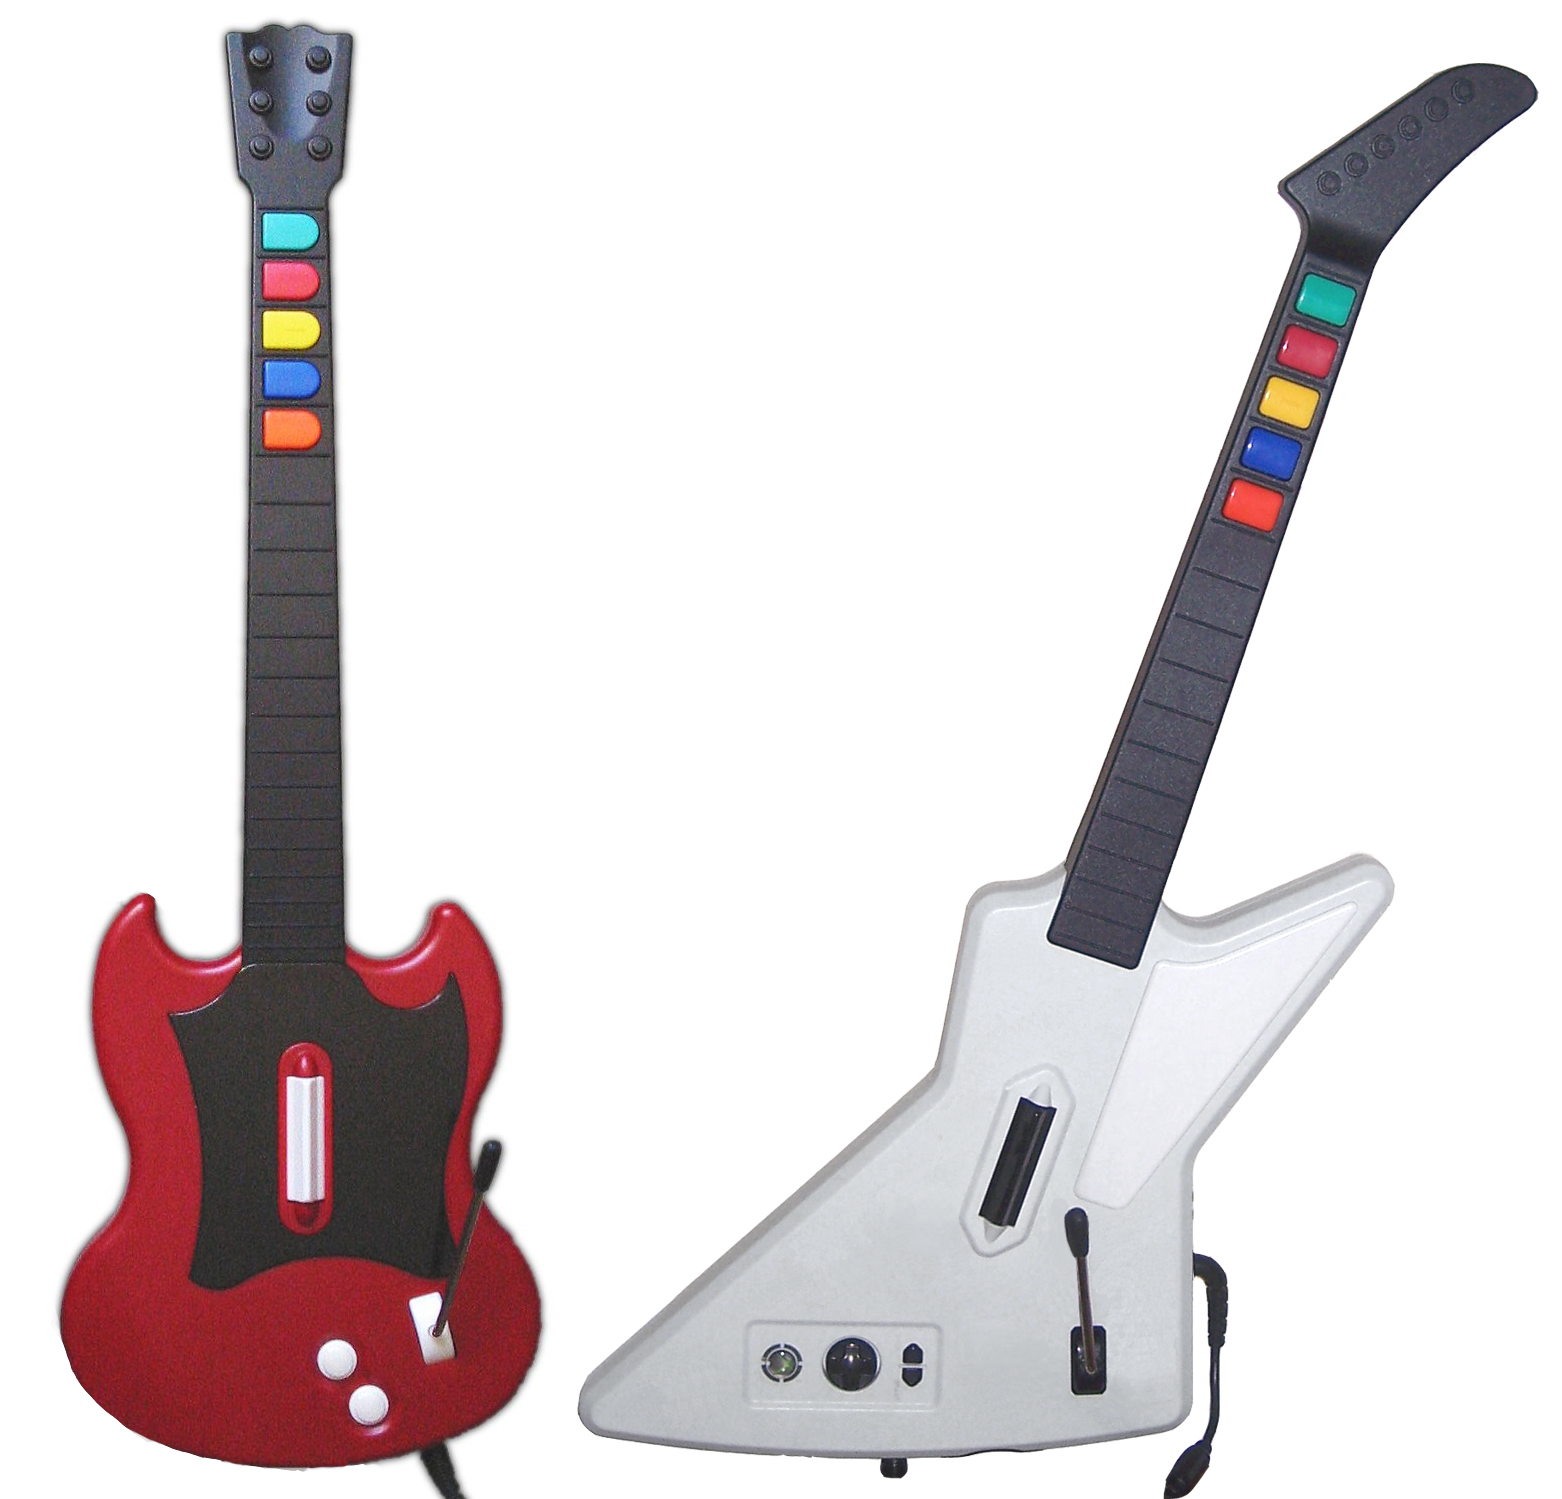
\includegraphics[width=0.43\textwidth]{Images/ExistingGames/GuitarHeroController.jpg}
    \end{center}
    \caption{Two different Guitar Hero controllers.}
    \label{fig:guitar_hero_controller}
\end{wrapfigure}

Guitar Hero is a series of games originally developed for PlayStation 2 in 2005. The game series later expanded to multiple other game platforms, including Xbox 360 and Nintendo Wii. The game concept is based on simulation and gamification of playing guitar, using a custom-developed guitar controller (see figure \ref{fig:guitar_hero_controller}). The player tries to match the in-game “notes” with buttons on the guitar controller, resulting in a score that is coherent with the number of notes hit. Songs available to choose from vary between different games, but generally, they belong to the genre of rock \cite{metacritic_guitar_2020}. Figure \ref{fig:guitar_hero_controller} shows a screenshot example from playing the game in single-player mode. 

One of the categories of alternative game characteristics is input. As per the definition (in chapter \ref{chap:5}), a game using alternative input sources can be classified as an alternative game. Guitar Hero is a typical example of such a game because it depends on a custom-designed controller for playing. Additionally, the use of gamification as the game genre is another reason why Guitar Hero can be defined as an alternative game. The main concept of the game can be viewed as gamification of playing guitar.

\begin{figure}[H]
    \centering
     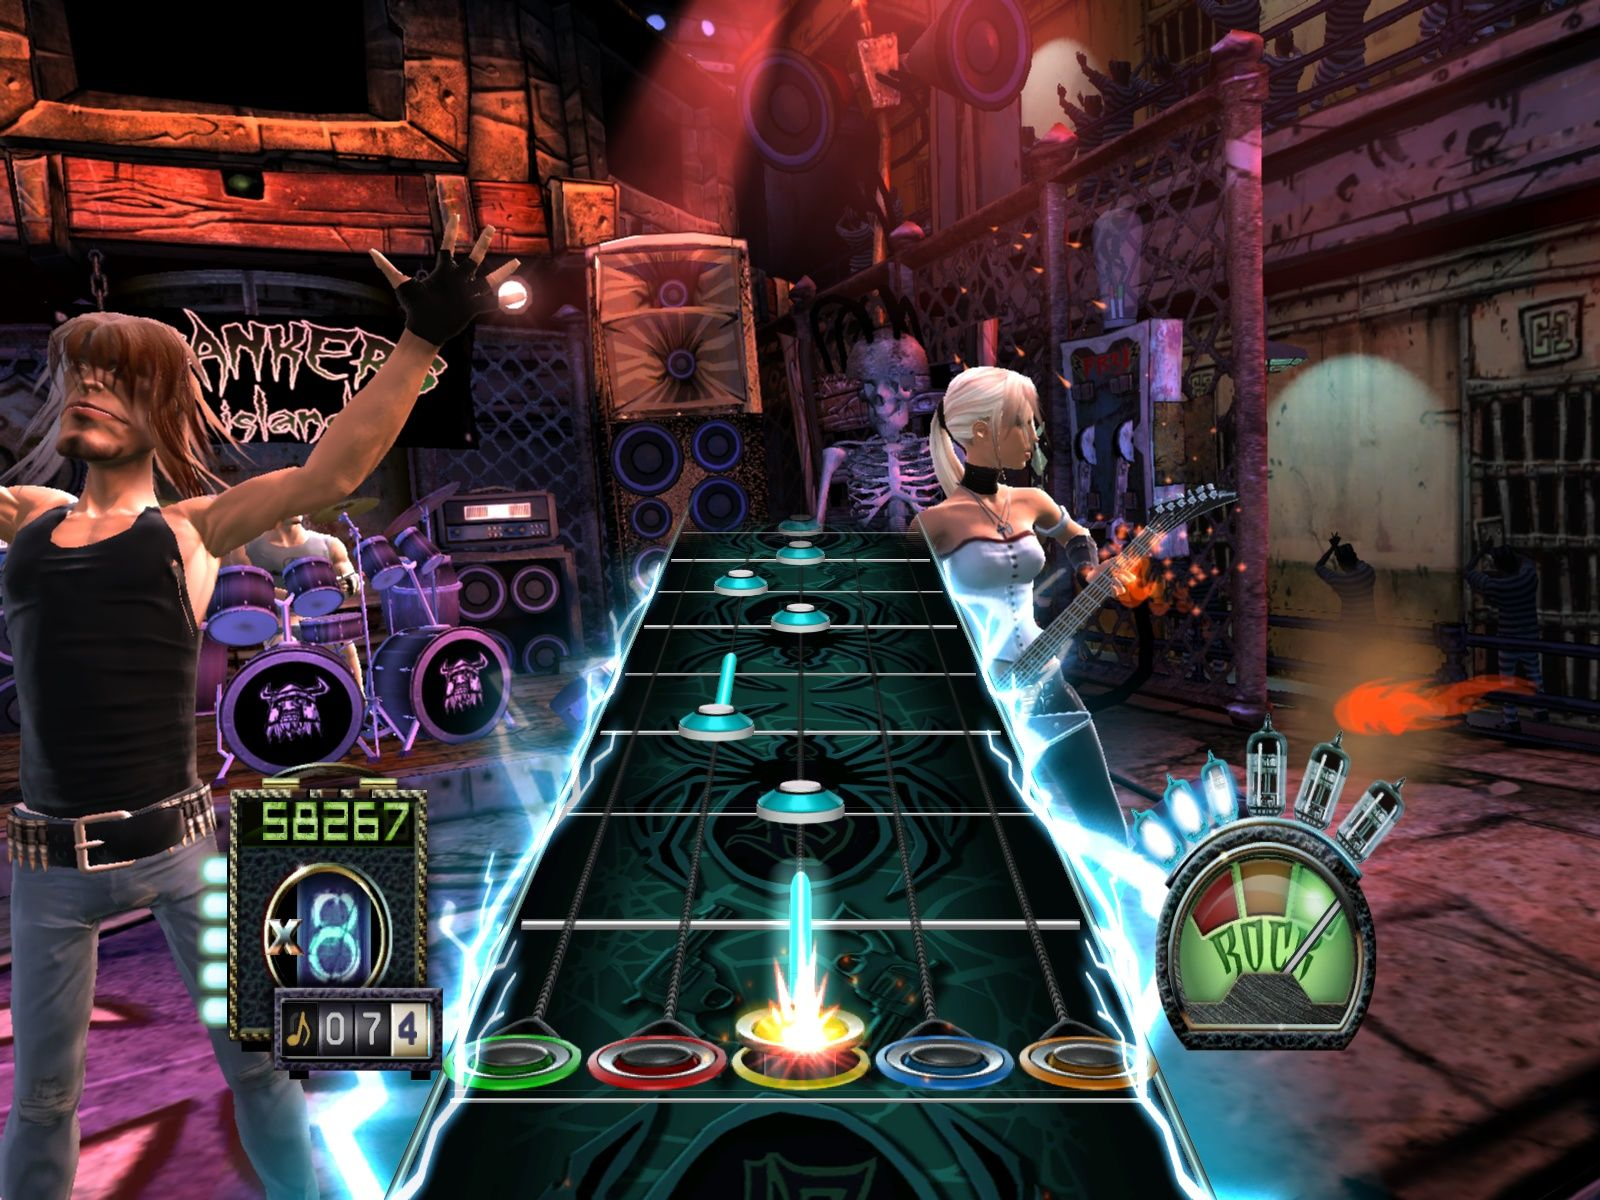
\includegraphics[width=0.8\textwidth]{Images/ExistingGames/GuitarHeroScreenshot.jpg}
    \caption{Screenshot from Guitar Hero gameplay.}
    \label{fig:guitar_hero_screenshot}
\end{figure}
        
\subsection{Wii Fit}
Wii Fit is an exercise game (exergame) created by Nintendo that launched in 2007 \citep{imdb_wii_2020}. The game is only available on Nintendo Wii and requires a special controller in addition to the regular Wii controller. Wii Fit is a collection of minigames that combine the two domains of health and entertainment. The game has four main exercise categories to choose from; strength training, aerobics, yoga, and balance \citep{ign_wii_2008}.

The additional controller is called the Wii Balance Board \citep{ign_wii_2008} and is one of the reasons that this game can be categorized as alternative. The board’s purpose is to track the user's movement and translate that to the user’s in-game avatar. The idea behind the board was drawn from the bathroom weight, and it consists of four weight sensors; one in each corner. The controller connects to the console through Bluetooth, where it calculates the user's movement in real-time \citep{jacquot_how_2010}. Based on the user’s movement, the game gives feedback on how the exercise is going.

In addition to the alternative input, Wii Fit is also a gamification of exercise. The goal of the game is to create a fun way of getting in shape from your own home. Nintendo is bringing a wide set of games that are engaging for the entire family with individual progress so all players can compare themselves against each other.

\begin{figure}[H]
    \begin{minipage}{.5\textwidth}
        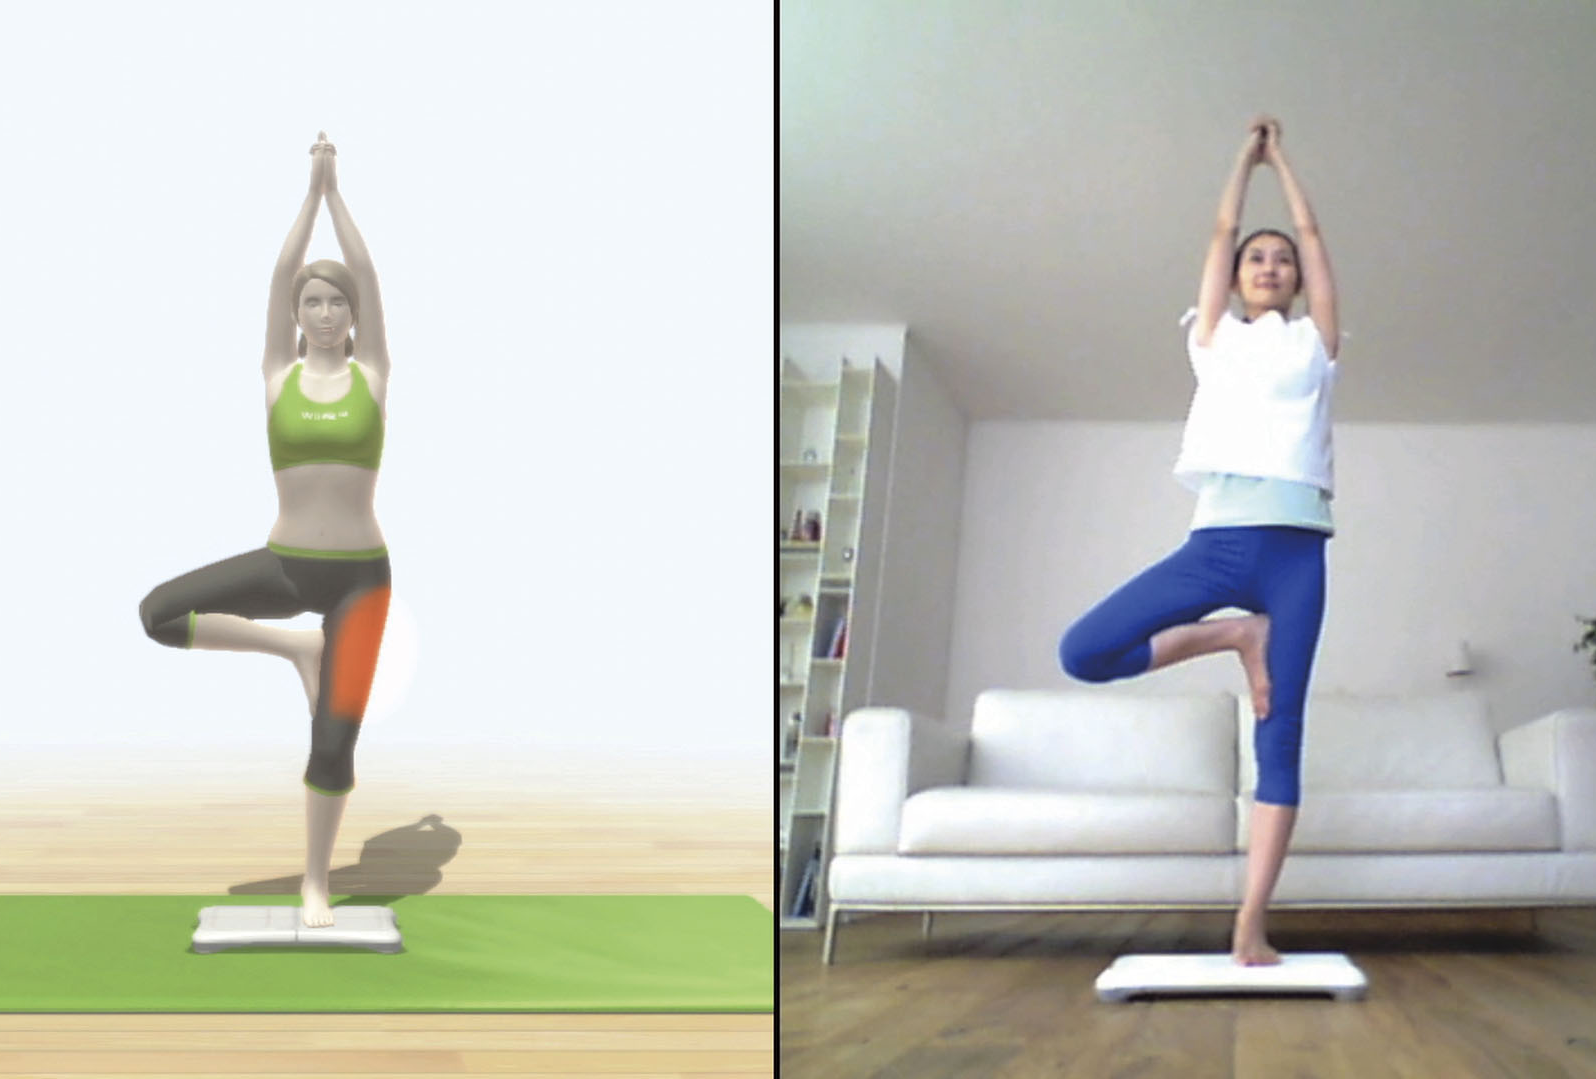
\includegraphics[width=0.95\textwidth]{Images/ExistingGames/WiiFit_Pose.png}
        \caption{Yoga exercise beside in-game avatar.}
        \label{fig:wii_fit_pose}
    \end{minipage}
    \hspace{0.5cm}
    \begin{minipage}{.5\textwidth}
        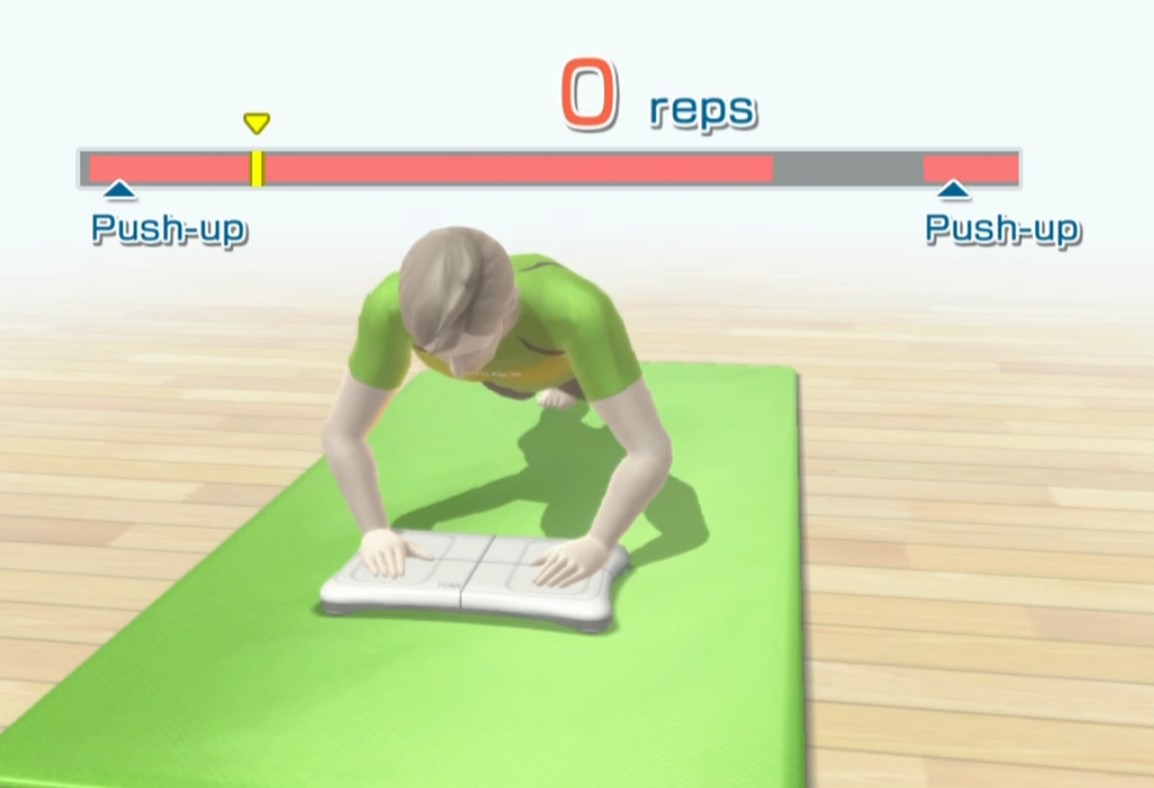
\includegraphics[width=0.95\textwidth]{Images/ExistingGames/WiiFit_Pushup.jpg}
        \caption{Screenshot of in-game avatar using the board to track push-ups.}
        \label{fig:wii_fit_pushup}
    \end{minipage}
\end{figure}

\subsection{Mosquito Mania}
Not written yet
    
\subsection{Comparison}
To be able to more easily compare the alternative aspects of all the games mentioned in this chapter, a model using the categories of characteristics presented in chapter \ref{chap:5} has been created. The model gives a quick overview of how the game differs and presents concrete characteristics for all the games in each of the six categories.

\begin{table}[H]
    \centering
    \begin{tabular}{lll}
        test & test & test \\
        test & test & test \\
        test & test & test
    \end{tabular}
    \caption{Existing alternative games characteristics comparison}
    \label{tab:existing_games}
\end{table}

\subsection{Model analysis}
The model in table \ref{tab:existing_games} is a simplified version of the complete model found in the Appendix \ref{appendix:complete_model}. The rows that have not been used, have been omitted for readability.

\subsection{Summary}
This chapter has focused on showcasing multiple different and typical examples of alternative games (based on our definition presented in chapter \ref{chap:5}). The examples have been shortly described and compared with each other to highlight their differences. A table with the characteristics of each game has been presented and analyzed. The next chapter will shift the focus from the concept of alternative games to the technical aspect of the field. 

\biblio % Needed for referencing to working when compiling individual subfiles - Do not remove
\end{document}